\section{问题三：有限侦听覆盖与有界收缩清除}

\subsection{模型与策略}

场地为闭圆盘$\mathbb A=\overline{\mathbb D}(0,1800)$。每个源的位置和频道固定，频道互异，源数$10\le N\le16$。对源$G$，有效接收半径$R_G\in[1000,1500]$；全向测量可听当且仅当检测点与源的距离不超过$R_G$。测向误差满足$|\alpha|\le1^\circ$，不要求独立、均匀或无偏，同一点重复测量也不被当作新信息。光学清除只要求距离不超过20 m；\texttt{near}表示距离不超过5 m，可以就地清除。

策略分为有限发现与有界清除两阶段。先处理原点及8个环点，每站完整扫描尚未发现的频道；仅在有严格覆盖证书时跳过该站。发现阶段不插入远距离追逐，以免覆盖任务被服务启发式反复推迟。然后对每个已发现且未清除的频道，使用示向度与距离上界逐步收缩，最后在保证进入20 m清除窗的位置清除。覆盖点的访问顺序用开放旅行商问题缩短路程，服务顺序按到下一收缩点的距离选择；这些顺序规则不改变完备性，也不声称求得全任务的全局最短时间。

虚拟时间按实际动作累加：
\begin{align}
\Delta T_{\rm measure}&=\|P_{\rm new}-P_{\rm old}\|/5
+\mathbf 1_{c\ne c_{\rm radio}}+5,\label{eq:tmeas}\\
\Delta T_{\rm clear}&=\|P_{\rm new}-P_{\rm old}\|/5+
\begin{cases}5,&\text{成功},\\3,&\text{未发现光学目标}.\end{cases}\label{eq:tclr}
\end{align}
修订算法的清除点均有距离证书，因此模型内应走成功分支；若接口返回失败，程序报告证书或模型异常，不把失败算成完成。现实程序时间与虚拟时间分别记录。

\subsection{9点侦听覆盖及其完整证明}

侦听点为
\begin{equation}
\mathcal N=\{O\}\cup\{R_k:k=0,\ldots,7\},\quad O=(0,0),\quad
R_k=1000(\cos(k\pi/4),\sin(k\pi/4)).\label{eq:q3net}
\end{equation}
定义最近站距离$d_{\mathcal N}(G)=\min_{S\in\mathcal N}\|G-S\|$。

\textbf{引理1（全向覆盖）。}在场地闭圆盘上，
\begin{equation}
\max_{G\in\mathbb A}d_{\mathcal N}(G)
=\rho=\sqrt{1800^2+1000^2-2\cdot1800\cdot1000\cos(\pi/8)}
\approx956.0511<1000.\label{eq:q3rho}
\end{equation}

\textbf{证明。}记$r=\|G\|$，$\delta\in[0,\pi/8]$为$G$与最近环点的夹角。令$\gamma=\cos(\pi/8)$、$\tau=1000/(2\gamma)\approx541.196$。若$r\le\tau$，选择原点即可使距离不超过$\tau<\rho$。若$\tau\le r\le1800$，选择最近环点$R$，由余弦定理，
\[
\|G-R\|^2=r^2+10^6-2000r\cos\delta
\le f(r):=r^2+10^6-2000\gamma r.
\]
$f$为凸函数，因此$f(r)\le\max\{f(\tau),f(1800)\}=\max\{\tau^2,\rho^2\}=\rho^2$。边界角平分点$P=1800(\cos(\pi/8),\sin(\pi/8))$到两相邻环点的距离均为$\rho$，到原点为1800，故上界可取到。证毕。

上述$r\le\tau$是证明中\emph{选择原点足以给出上界}的区间，不是所有方向上的最近站分界。固定$\delta$时，原点与最近环点等距的半径是$1000/(2\cos\delta)$；例如$G=(520,0)$的最近环点距其480 m，比原点近。另须区分覆盖半径：8个环点在原点的最近距离为1000 m，所以它们不能以$\rho$为半径覆盖原点，但可以用闭1000 m盘覆盖原点；事实上8环以闭1000 m盘已覆盖场地。保留原点扫描利用了题设初始位置，且使最大最近距离降至$\rho$。

\begin{figure}[htbp]
\centering
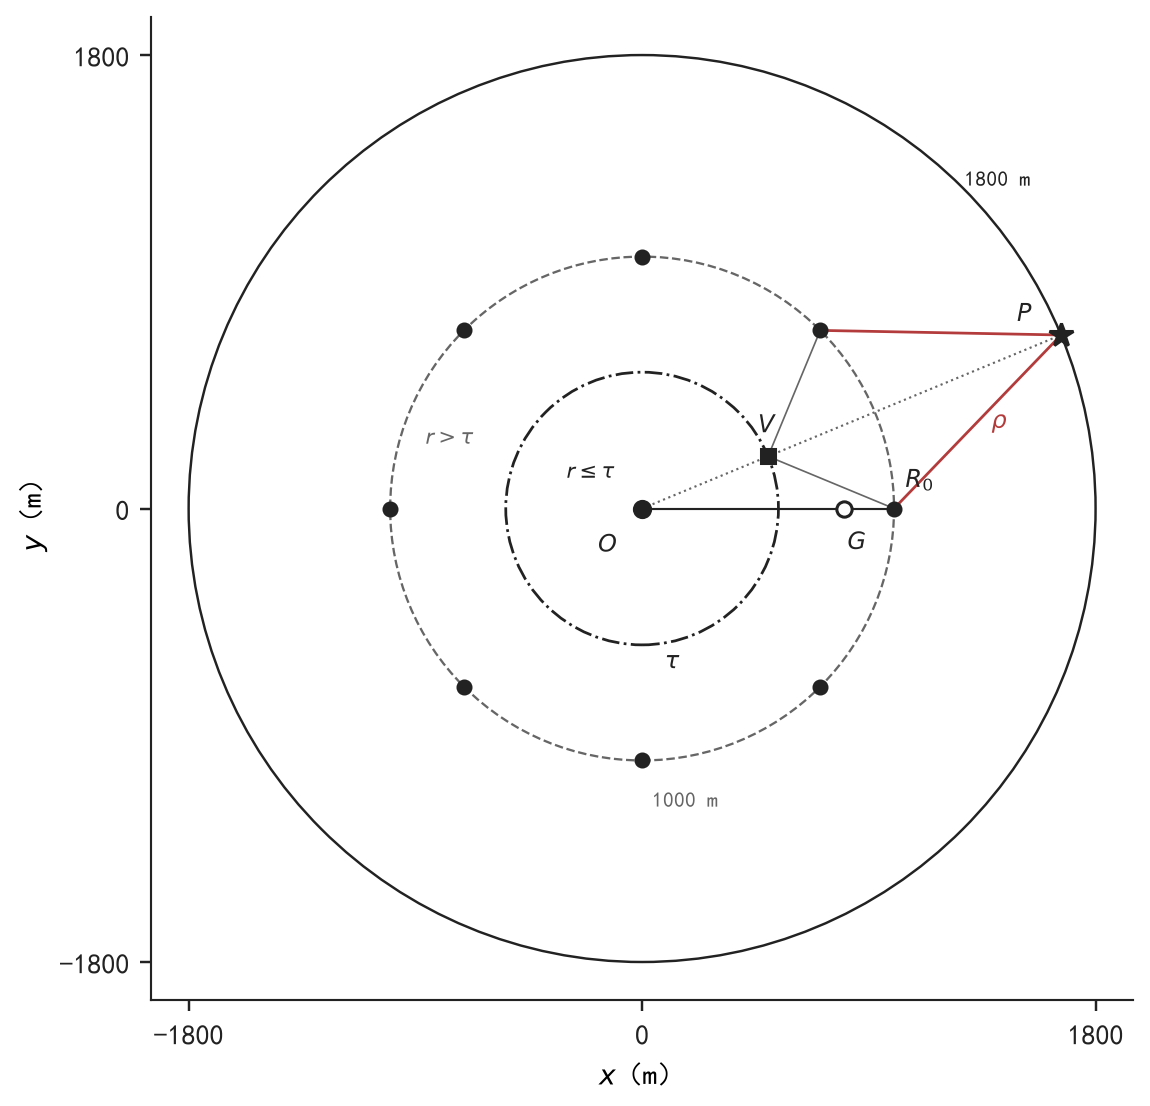
\includegraphics[width=0.59\textwidth]{figures/q3_nine_disk.png}
\caption{9点覆盖几何。实线圆为场地，虚线圆为环点所在圆，点划线半径$\tau$是证明分段界，不是圆形Voronoi胞腔。$V$是Voronoi顶点，$P$取到最远距离$\rho$。8环可用闭1000 m盘覆盖原点，但不能用半径$\rho$覆盖原点。}
\label{fig:ninedisk}
\end{figure}

\begin{table}[htbp]
\centering
\caption{问题三侦听点坐标（计算使用未取整坐标）}\label{tab:q3xy}
\begin{tabular}{crrl}\toprule
编号 & $x$/m & $y$/m & 角色\\\midrule
1 & 0 & 0 & 原点\\
2 & 1000 & 0 & 环$k=0$\\
3 & 707.1 & 707.1 & 环$k=1$\\
4 & 0 & 1000 & 环$k=2$\\
5 & $-707.1$ & 707.1 & 环$k=3$\\
6 & $-1000$ & 0 & 环$k=4$\\
7 & $-707.1$ & $-707.1$ & 环$k=5$\\
8 & 0 & $-1000$ & 环$k=6$\\
9 & 707.1 & $-707.1$ & 环$k=7$\\\bottomrule
\end{tabular}
\end{table}

\subsection{连续残留与可验证的保守剪枝}

设$\mathcal S$是实际\emph{完整且成功}扫描过当时所有静默频道的站点集合。定义
\begin{equation}
\mathrm{Res}_{\rm cont}(\mathcal S)=\mathbb A\setminus
\bigcup_{S\in\mathcal S}\overline{\mathbb D}(S,1000),\qquad
K_Q=\overline{\mathbb D}(Q,1000)\cap\mathbb A.\label{eq:rescont}
\end{equation}
任何尚未发现的源都属于该残留：若它距某发现站不超过1000 m，该站已经测量其频道，必然发现它。因而$K_Q$被已有发现站的1000 m盘覆盖时，可免去该覆盖义务。

\textbf{引理2（安全跳过）。}若$Q\in\mathbb A$且$K_Q\subseteq\bigcup_{S\in\mathcal S}\overline{\mathbb D}(S,1000)$，则$Q$不能听到尚未发现的源，即使该源的实际接收半径超过1000 m。

\textbf{证明。}假设$Q$能听到未发现源$G$，记$d=\|Q-G\|\le R_G$。若$d\le1000$，则$G\in K_Q$，与其未发现矛盾。若$d>1000$，在线段$QG$上取$\|Q-P\|=1000$。场地凸性保证$P\in K_Q$，故存在发现站$S$使$\|S-P\|\le1000$。于是$\|S-G\|\le1000+(d-1000)=d\le R_G$，该站本应听到$G$，仍矛盾。证毕。

在精确几何中，跳过等价于$\rho(\mathcal S,K_Q)=\max_{p\in K_Q}\min_{S\in\mathcal S}\|p-S\|\le1000$。用Voronoi顶点、边与边界圆交点、径向极值和透镜顶点枚举可以研究该最大值，但普通浮点枚举值不是自动带误差保证的上界。将判定阈值放宽为$1000+10^{-9}$同样不构成严格证书。

修订实现采用有理数矩形细分证书。将输入浮点数精确转换成其二进制有理数值，从包含$K_Q$的矩形开始，对每个矩形$B$执行：
\begin{enumerate}
\item 若$B$到某约束圆心的最小距离平方严格大于该圆半径平方，则$B$不与$K_Q$相交，可排除。
\item 若$B$四个角到某发现站的最大距离平方不超过$1000^2$，则整个矩形被该站覆盖，可认证。
\item 否则沿较长边对半细分；达到256个处理矩形的计算上限仍未结束，则返回“未认证”，保留侦听点。
\end{enumerate}
有限个已认证矩形覆盖所有可能与$K_Q$相交的区域，才能返回真。这里检查的是整块矩形的严格上界，不是有限点采样。若某约束圆盘本身已包含于一个发现站盘中，则用圆盘包含关系直接认证，特别覆盖扫描过的同中心盘。缓存使用原始坐标，不作六位小数舍入。证书不完备只会增加扫描，不会遗漏源。

原实现还使用内接正多边形裁剪场地和接收圆盘，可能切掉位于真实圆弧上的源，因此小多边形的包围圆不能直接当作真实可行集的清除证书。修订Q3的默认路径不使用该近似来决定清除；若进一步引入交会加速，应使用包含真实圆盘的外近似，并证明数值误差方向。

有限采样反例仍然成立。取$R_G=1000$，$G_\star=1800(\cos(\pi/24),\sin(\pi/24))$。其到$R_0$约819.023 m，到其余网点至少1176.405 m；八个边界角平分样本却可以全被其余网点覆盖。因此有限样本已空不能证明连续残留为空。反例明确取最小接收半径，不将“距其它站超过1000 m”误写成对所有$R_G$均不可听。

\subsection{距离上界收缩与有限步清除}

第一次得到\texttt{direction}时，只知道源位于该测向楔内且距离不超过1500 m。无须知道真实距离，也无须假设首次发现站是最近网点。

\textbf{引理3（半上界步进）。}在$S$测得单位示向度向量$u$，且已知$\|G-S\|\le R\le1500$。取
\begin{equation}
P=S+\frac R2u,\qquad \kappa=\sqrt{\frac54-\cos1^\circ}\approx0.5001523.
\label{eq:q3contract}
\end{equation}
则$\|G-P\|\le\kappa R$，且$\kappa R\le750.229<1000$，因此在$P$对该全向源测量必返回\texttt{direction}或\texttt{near}。

\textbf{证明。}记$r=\|G-S\|\in[0,R]$，误差$|\alpha|\le1^\circ$。余弦定理给出
\[
\|G-P\|^2=r^2+\frac{R^2}{4}-rR\cos\alpha
\le r^2+\frac{R^2}{4}-rR\cos1^\circ.
\]
右侧关于$r$凸，在$[0,R]$上的最大值位于端点，故不超过
$\max\{R^2/4,(5/4-\cos1^\circ)R^2\}=\kappa^2R^2$。
由于$R_G\ge1000$，新点仍可听。证毕。该论证逐步适用于任意允许误差序列，不依赖误差的概率分布。

代码使用更宽的收缩系数$\bar\kappa=0.501$，并采用递推
\begin{equation}
R_0=1500,\qquad R_{j+1}=0.501R_j+10^{-6}\quad (\mathrm m),
\label{eq:q3bound}
\end{equation}
同时向上取浮点相邻数，给坐标和三角函数运算留外向裕量。第$j+1$点仍取$S_j+(R_j/2)u_j$，不将坐标投影回场地圆盘；题目允许场地外检测。前六步若未返回\texttt{near}，在新点测量并更新示向度；第七步有$R_7<12<20$，直接清除，不再测量。若中途\texttt{near}则在该点清除。每源在首次发现后最多用六次测量加一次清除，共7次接口动作。

\begin{table}[htbp]
\centering
\caption{收缩清除的距离上界（按式\eqref{eq:q3bound}，向上显示）}
\label{tab:q3contraction}
\begin{tabular}{crl}\toprule
步数 & 上界/m & 动作\\\midrule
0 & 1500.000 & 已有首次示向度\\
1 & 751.501 & 测量；\texttt{near}则清除\\
2 & 376.502 & 测量；\texttt{near}则清除\\
3 & 188.628 & 测量；\texttt{near}则清除\\
4 & 94.503 & 测量；\texttt{near}则清除\\
5 & 47.346 & 测量；\texttt{near}则清除\\
6 & 23.721 & 测量；\texttt{near}则清除\\
7 & 11.884 & 直接清除\\\bottomrule
\end{tabular}
\end{table}

这一距离证书与问题一的包围圆证书一致：只要$G\in\Omega\subseteq\overline{\mathbb D}(C,20)$，在$C$清除就充分；不必先求出真实坐标或把多楔交压到20 m。相应地，若$G\in\Omega$且最小包围圆半径不超过1000 m，在其圆心再测对全向源可听。原先的轴上弦长$2r\sin(|\alpha|/2)$只适用于清除点轴向距离恰为未知真实距离$r$的构造，不是修订程序的步长规则，也不再承担可执行性证明。

\subsection{完整算法、动作上界与终止语义}

\begin{enumerate}
\item 成功\texttt{/enter}后，从返回值建立现实时间截止时刻；预留退出动作。先在原点测量所有静默频道，\texttt{near}就地清除，其余读数存储。
\item 剩余8个环点按当前位姿的开放TSP访问。每次取出一个环点；若其透镜有严格覆盖证书则跳过，否则完整扫描静默频道。仅在全部请求被接受、响应有效后，将该站加入发现集合。
\item 剩余环点为空、已发现16个不同频道，或静默频道为空时结束发现阶段。未知源数量不通过连续多次空扫来猜测。
\item 在已发现但未清除的频道中，选到其第一收缩点最近者，按引理3服务；完成后重新选择下一频道。无需先返回存储示向度的旧站，源位置固定保证旧读数仍有效。
\item 仅当发现已完成且所有已发现频道均收到成功清除响应时，输出\texttt{complete=true}。预算、超时、拒绝、无效响应、收缩点无信号或证书清除失败均输出明确未完成原因。
\end{enumerate}

\textbf{定理（Q3有限动作清除）。}在题设的全向、固定源、误差和接收半径条件下，若各请求在现实测试期限内正常接受并执行，则上述算法清除所有源。计入进入和退出，接口动作不超过
\begin{equation}
A\le1+9\cdot20+7N+1\le294<900.\label{eq:q3actions}
\end{equation}

\textbf{证明。}引理1保证每个源位于至少一个原始网点的1000 m盘内；引理2保证剪掉的透镜已由完整扫描覆盖。每轮处理并永久移除一个环点，最多8轮，不存在服务点反复插入造成的覆盖饥饿。若提前听满16个，由$N\le16$也已发现全部源。故发现阶段最多$9\cdot20$次测量。引理3保证每个已发现源最多7次服务动作后清除；发现时的\texttt{near}清除计入对应源的这7次额度。再计进入、退出各一次即得上界。证毕。

900是程序自设动作闸，并非原题常数。与只证明“正常结束时已发现”的命题相比，本定理给出模型内有限动作上界，因而默认动作闸不会截断有效轨迹。但动作数不等于现实用时，网络延迟、计算耗时、20分钟程序期限、25分钟窗口及技术异常仍可能使实际运行未完成；定理不把这些外部中断当作成功。

虚拟100小时上限也不会在模型内触发。覆盖段至多8次网点间移动，粗界16000 m。每条收缩链的相邻计划点总长小于1504 m，服务点到原点的距离不超过2504 m；从上一服务终点到下一第一收缩点的距离可粗界为4254 m。每源服务路程因此小于5758 m，全任务总路程小于110 km，移动与检测清除虚拟时间合计小于7小时。这只是保守可行性界，不是平均时间估计。开放TSP只精确优化当前覆盖站点的路程；未知源位置和后续服务仍使用启发式顺序。

\subsection{验证结果与历史演练的区分}

\begin{table}[htbp]
\centering
\caption{修订Q3的独立离线模型验证（非官方模拟器）}\label{tab:q3offline}
\begin{tabular}{lr}\toprule
量 & 结果\\\midrule
场景数 / 全清场景数 & 48 / 48\\
每场源数 & 10--16\\
动作次数范围（含进入退出） & 150--245\\
理论动作上界 & 294\\
总虚拟时间/总清除数（s/源） & 434.228\\
场均路程（m） & 22839.8\\
官方模拟器演练次数（修订代码） & 0\\\bottomrule
\end{tabular}
\end{table}


新代码的离线验证由\texttt{code/q3/offline\_validation.py}复现，随机种子从20260913起，共48个场景，源数循环取10至16。位置类型包含均匀圆盘、边界、聚簇及回归构型；误差类型包含恒定$+1^\circ$、恒定$-1^\circ$、零误差、随位置固定的有界误差和随位置固定的端点误差。回归构型含$G_\star$、原点近源及$(1400,0)$处接收半径1500 m的首次远距离发现。算法仅通过模拟客户端的测量与清除响应决策，测试器另用真值检查每一个收缩距离上界。

这些是按题设建立的独立离线模型测试，不是官方模拟器演练，不产生正式案例编码。完整结果和种子见\texttt{code/q3/offline\_results.json}。单元测试另覆盖亚微米和亚纳米剪枝反例、同心边界、细分预算耗尽、部分扫描被拒、动作预算、现实期限和证书清除失败；这些测试用于检查实现，不代替上述证明。

原包保留三次历史演练数据，见表\ref{tab:q3reh}。对应的是原覆盖骨架与射线启发式，原代码另存为\texttt{searcher\_legacy.py}。三次总虚拟时间除以总清除数的加权平均为
\[
\frac{3158.7139+3360.202868+3245.032067}{16+12+11}
\approx250.358\ \text{s/源}.
\]
该统计不等于三个案例均值的算术平均，也不是修订算法的速度。原包未提供足以重放这些案例的完整明文轨迹，故本次仅核对表格算术，不声称重新验证了这些官方演练结果。新旧场景不配对，不能据此宣称修订策略加速或减速。

\begin{table}[htbp]
\centering\scriptsize
\caption{原包历史Q3演练统计（旧启发式；不是修订代码成绩或正式测试）}\label{tab:q3reh}
\begin{tabular}{llrrrrr}\toprule
演练 & 案例编码 & 总数 & 清除 & 比例 & 动作 & 平均时间/s\\\midrule
1 & UUDJ-WJGP-NBRH-8V2N & 16 & 16 & 1.000 & 132 & 197.42\\
2 & XUXT-9646-NF9K-42J4 & 12 & 12 & 1.000 & 150 & 280.02\\
3 & 2GA6-9ADV-XD3E-AVMK & 11 & 11 & 1.000 & 160 & 295.00\\\bottomrule
\end{tabular}
\end{table}

原文另外列出24个旧同构场景全部清除、均值272.227 s/源、动作123至213的汇总；原包不含逐场景记录与对应测试器，本次不将其作为可复现的新验证结果。

\begin{figure}[htbp]
\centering
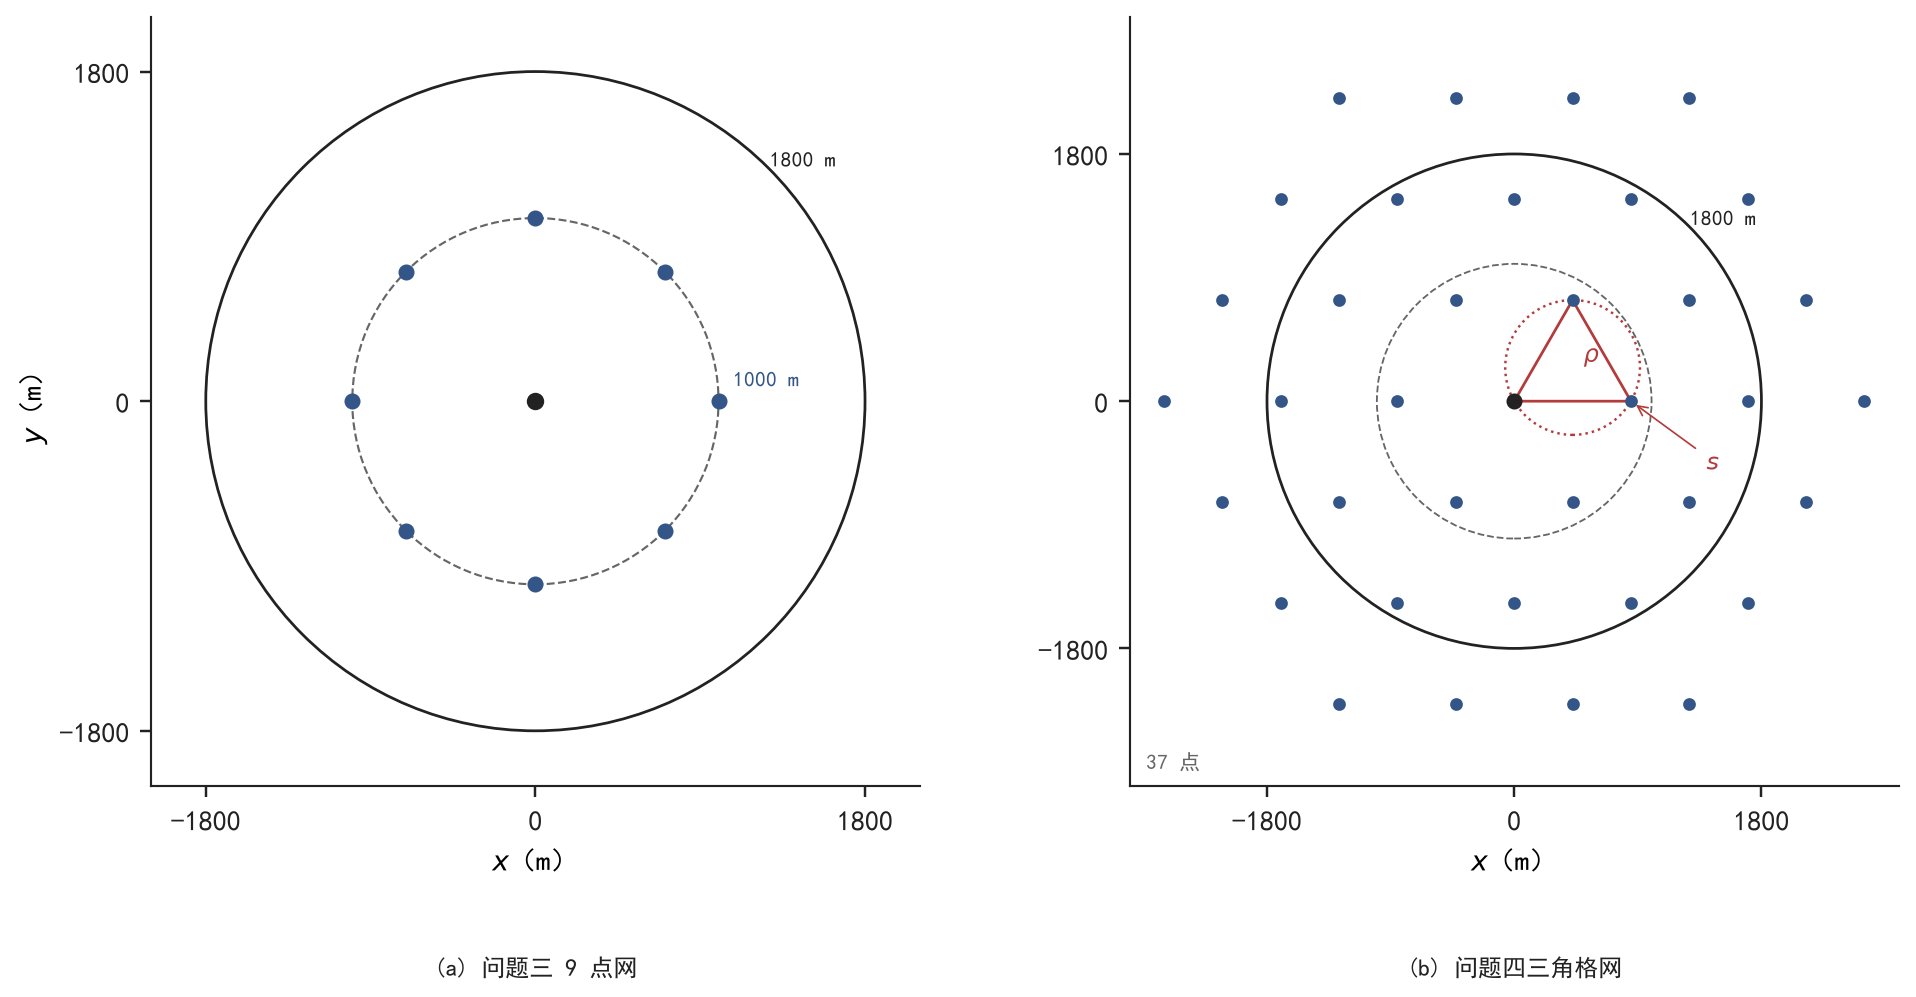
\includegraphics[width=0.94\textwidth]{figures/q34_scout_nets.png}
\caption{左：Q3原点加8环的侦听网；右：原文Q4三角格网。两问的方向假设不同，Q3收缩清除证明不能直接用于Q4。}\label{fig:scouts}
\end{figure}
\begin{figure}[htbp]
\centering
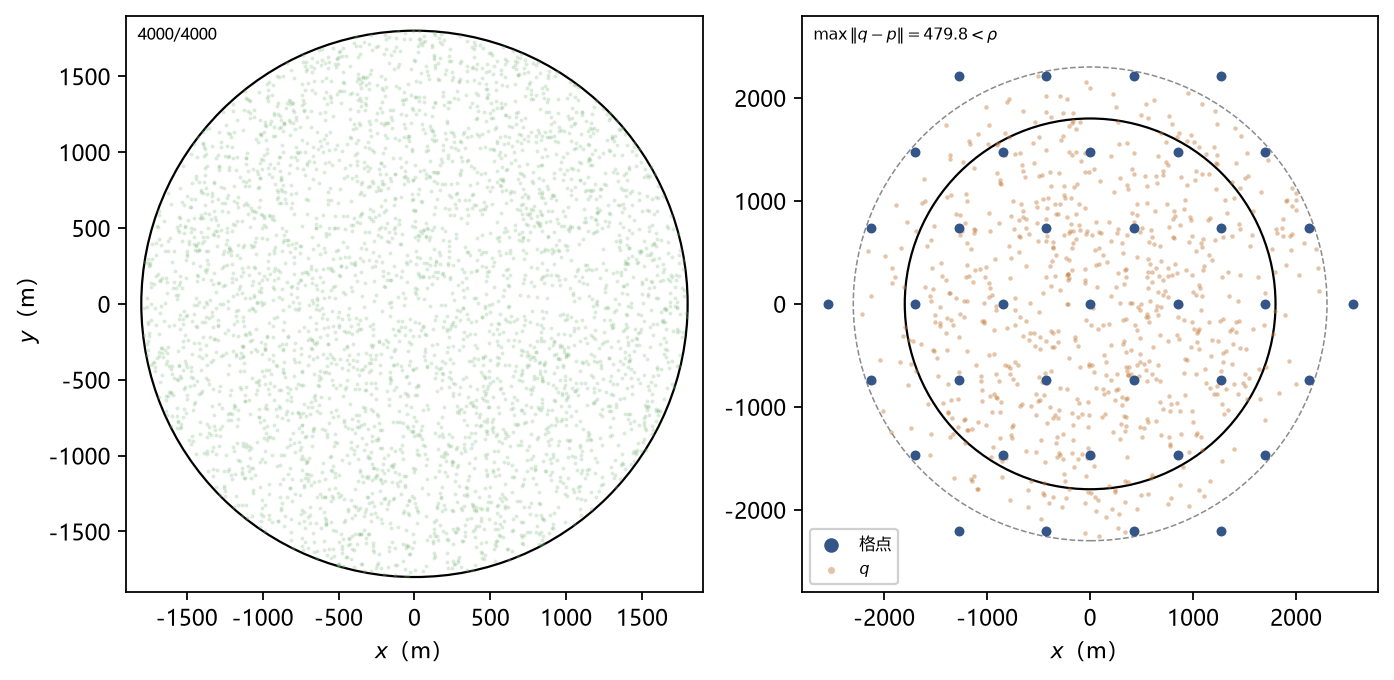
\includegraphics[width=0.94\textwidth]{figures/q34_coverage_scatter.png}
\caption{原包几何采样示意：左为Q3的4000个圆盘样本，右为Q4平移点与格点。采样图只作示意，Q3全称覆盖由引理1证明。}\label{fig:covmap}
\end{figure}

\subsection{正式测试与适用边界}

题目要求的三次正式测试尚无可核验数据。表\ref{tab:official3}保留题目表1的四个字段，测试序号写入案例编码栏；不得用旧演练或新离线结果补填。修订算法仍需在官方模拟器中演练，并导出三次正式日志，才能完成题目要求的实测交付。

\begin{table}[htbp]
\centering
\caption{问题三正式测试结果（待官方测试填写）}\label{tab:official3}
\begin{tabular}{lccc}\toprule
测试案例编码 & 清除干扰源个数 & 平均定位清除时间 & 程序运行时间\\\midrule
测试1：待测试 & --- & --- & ---\\
测试2：待测试 & --- & --- & ---\\
测试3：待测试 & --- & --- & ---\\\bottomrule
\end{tabular}
\end{table}

该算法提供有明确动作上界的可行解。它没有证明全任务时间最优；保守初始距离上界可能产生额外移动。今后的交会和D-最优加速应只减少已认证工作，或在有限预算内回退到本节的收缩步骤，不能重新引入无证书剪枝、以\texttt{no\_signal}猜测越源、或无上界的服务循环。所有结论限于Q3全向源，未将定向瓣的无信号解释成单纯超距。
\FloatBarrier
